\section{Interprocedural Profiling}

The first contribution we present in this thesis is an {\em interprocedural} technique for identifying the calling context that are most frequently encountered across function invocations at run-time. We show that the traditional approach for constructing a {\em Calling Context Tree} (CCT) might not be sustainable for real-world applications, as their CCTs often consist of tens of millions of nodes, making them difficult to analyze and also hurting execution time because of poor access locality. We thus introduce a novel data structure, the {\em Hot Calling Context Tree} (HCCT), in the spectrum of representations for interprocedural control flow. The HCCT is defined as the subtree of the CCT containing only its most visited nodes, which we call {\em hot}, along with their ancestors, and can be constructed independently of the CCT using fast, space-efficient algorithms for mining frequent items in data stream.

\subsection{Motivation and Contributions}
The dynamic {\em calling context} of a routine invocation is defined as the sequence of functions that are concurrently active on the run-time stack. A calling context leads to an exact program location, as it corresponds to the sequence of un-returned calls from a program’s root function to the routine invocation it is associated with.

Context-sensitive profiling information provides valuable information for program understanding, performance analysis, and runtime optimizations. Previous works demonstrated its effectiveness for tasks such as residual testing~\cite{PavlopoulouY99,Vaswani07}, function inlining~\cite{Chang92}, statistical bug isolation~\cite{Feng03,Liblit03}, performance bug detection~\cite{Nistor13}, object allocation analysis~\cite{Nethercote07}, event logging~\cite{Zhang06}, or anomaly-based intrusion detection~\cite{Bond07}.
% this is a sync with PCCE paper
Calling-context information can also be employed in unit test generation~\cite{Villazon09}, testing of sensor network applications~\cite{Lai08}, and reverse engineering of protocol formats~\cite{Lin08}.

\begin{table}[ht]
\begin{small}
\ifauthorea{}{\centering}
\begin{tabular}{|l|r r r r|}
\hline
Application & $|$Call graph$|$ & Call sites & $|$CCT$|$ & $|$Call tree$|$\\
\hline
amarok & 13\,754 & 113\,362 & 13\,794\,470 & 991\,112\,563 \\
ark & 9\,933 & 76\,547 & 8\,171\,612 & 216\,881\,324 \\
audacity & 6\,895 & 79\,656 & 13\,131\,115 & 924\,534\,168 \\
bluefish & 5\,211 & 64\,239 & 7\,274\,132 & 248\,162\,281 \\
dolphin & 10\,744 & 84\,152 & 11\,667\,974 & 390\,134\,028 \\
firefox & 6\,756 & 145\,883 & 30\,294\,063 & 625\,133\,218 \\
gedit & 5\,063 & 57\,774 & 4\,183\,946 & 407\,906\,721 \\
ghex2 & 3\,816 & 39\,714 & 1\,868\,555 & 80\,988\,952 \\
gimp & 5\,146 & 93\,372 & 26\,107\,261 & 805\,947\,134 \\
gwenview & 11\,436 & 86\,609 & 9\,987\,922 & 494\,753\,038 \\
inkscape & 6\,454 & 89\,590 & 13\,896\,175 & 675\,915\,815 \\
oocalc & 30\,807 & 394\,913 & 48\,310\,585 & 551\,472\,065 \\
ooimpress & 16\,980 & 256\,848 & 43\,068\,214 & 730\,115\,446 \\
oowriter & 17\,012 & 253\,713 & 41\,395\,182 & 563\,763\,684 \\
pidgin & 7\,195 & 80\,028 & 10\,743\,073 & 404\,787\,763 \\
quanta & 13\,263 & 113\,850 & 27\,426\,654 & 602\,409\,403 \\
sudoku & 5\,340 & 49\,885 & 2\,794\,177 & 325\,944\,813 \\
vlc & 5\,692 & 47\,481 & 3\,295\,907 & 125\,436\,877 \\
%\hline
botan & 3\,388 & 27\,114 & 308\,550 & 26\,272\,804\,980 \\
cairo-perf-trace & 1\,408 & 3\,696 & 137\,920 & 15\,976\,619\,734 \\
crafty & 107 & 516 & 36\,434\,095 & 10\,403\,074\,070 \\
fhourstones & 18 & 32 & OOM & 39\,272\,563\,944 \\
gobmk & 1\,133 & 4\,049 & OOM & 21\,909\,088\,291 \\
ice-labyrinth & 2\,335 & 8\,050 & 2\,160\,052 & 1\,637\,076\,406 \\
mount-herring & 2\,318 & 8\,269 & 3\,733\,120 & 3\,311\,257\,932 \\
overworld & 14\,173 & 50\,394 & 3\,774\,937 & 4\,112\,679\,880 \\
scotland & 13\,932 & 51\,206 & 1\,813\,368 & 5\,982\,612\,379 \\
sjeng & 57 & 221 & OOM & 28\,370\,207\,811 \\
\hline
\end{tabular}
\vspace{4mm}
\caption{\label{tab:hcct-CCTsize} Number of nodes of call graph, call tree, calling context tree, and number of distinct call sites for different applications. OOM stands for {\em Out Of Memory} (i.e., the CCT is too large to be constructed in main memory on a 32-bit architecture). Game PlanetPenguin Racer has been run on courses {\tt mount-herring} and {\tt ice-labyrinth}; similarly, game SuperTuxKart has been run on tracks {\tt overworld} and {\tt scotland}. }
\end{small}
\end{table}
\ifauthorea{\newline}{\vspace{-6mm}}

\mynote{Add reference to related work section for the CCT}
Calling context trees (CCTs) offer a compact representation for context-sensitive information. In fact, a CCT yields a more accurate profile than a {\em call graph} (which can sometimes drive to misleading conclusions~\cite{Ponder88, Spivey04}) in a space that is typically several orders of magnitude smaller than the one required to maintain a {\em call tree}. Many techniques have also been proposed over the years to reduce the overhead for its construction.
%, by trading accuracy for performance.

However, even CCTs may be very large and difficult to analyze in several applications~\cite{Bond07,Zhuang06}; their sheer size might also hurt execution time, because of poor access locality during construction and query. As an example, we report in \mytable\ref{tab:hcct-CCTsize} numbers collected for short usage sessions of off-the-shelf Linux applications and for benchmarks from popular suites. Under the optimistic assumption that each CCT node requires 20 bytes for its representation on a 32-bit architecture\footnote{From maintaining routine ID, its call site, and a performance metric as {\tt int} fields, along with two pointers for a first-child, next-sibling representation. Previous works~\cite{Ammons97,Spivey04} use larger nodes.}, nearly 1 GB of memory is needed just to maintain OpenOffice Calc's 48-million-node CCT.

In a performance profiling scenario, we remark that only the most frequent contexts are of interest, as they represent the hot spots to which optimizations must be directed. As observed in~\cite{Zhuang06}: ``Accurately collecting information about hot edges may be more useful than accurately constructing an entire CCT that includes rarely called paths.'' \myfigure\ref{fig:hcct-skewness} shows that, for different applications, only a small fraction of contexts are hot: in conformance with the Pareto principle, nearly 90\% of routine calls take place in only 10\% of contexts. The skewness of the distribution suggests that space could be greatly reduced by keeping information about hot contexts only and discarding on the fly likely cold (i.e., having low frequency) contexts.

\ifdefined\noauthorea
\begin{figure}[hb]
\begin{center}
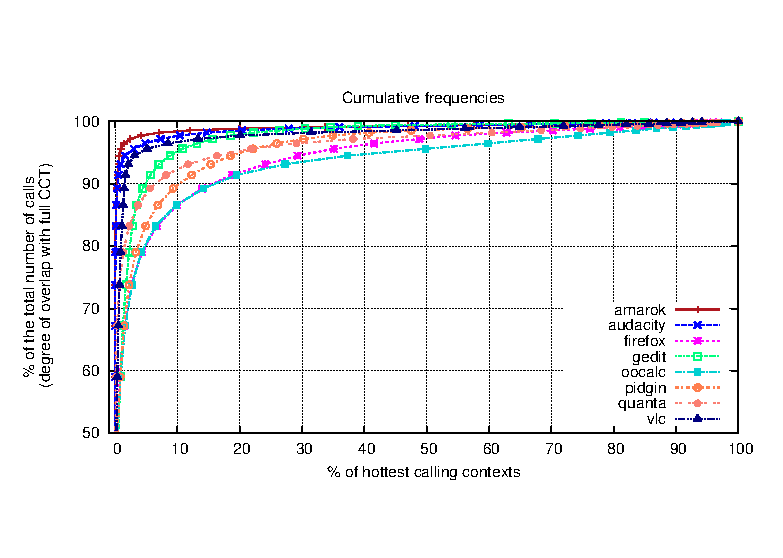
\includegraphics[width=0.95\columnwidth]{figures/hcct-skewness/hcct-skewness.eps}
\caption{\protect\label{fig:hcct-skewness} Skewness of calling contexts distribution on a representative subset of applications. For instance, in {\tt oocalc}, 10\% of the hottest calling contexts account for more than 86\% of all routine calls.
}
\end{center}
\end{figure}
\fi

\paragraph*{Contributions.} In this thesis, we introduce a novel run-time data structure, called {\em Hot Calling Context Tree (HCCT)}, that compactly represents all the hot calling contexts encountered during a program's execution, offering an additional intermediate point in the spectrum of data structures for representing interprocedural control flow. The HCCT is a subtree of the CCT that includes only hot nodes and their ancestors, also maintaining estimates of performance metrics (e.g., frequency counts) for hot calling contexts. We cast the problem of identifying the most frequent contexts into a data streaming setting: we show that the HCCT can be computed without storing the exact frequency of all calling contexts, by using fast and space-efficient algorithms for mining frequent items in data streams. These algorithms allow us to distinguish between hot and cold contexts on the fly, with the accuracy of maintained frequency estimates being formally guaranteed.

%Context-sensitive profiling provides 
%These algorithms allow us to distinguish between hot and cold context on-the-fly, and we show both theoretically and experimentally that for collected metrics the HCCT achieves a similar precision as the CCT in a space that is several orders of magnitude smaller. We show on prominent benchmarks that our implementation, shipping as a plugin for the \gcc\ compiler, incurs a slowdown competitive with the \gprof\ profiler while collecting much finer-grained profiles.

\subsection{Approach}
\label{ss:hcct-approach}

\paragraph*{Calling Context Trees.} A {\em calling context tree} (CCT) can be used to compactly represent all calling contexts encountered during the execution of a program. Calling contexts can be straightforwardly mapped to paths in a tree: nodes represent un-returned function calls, and each path from the root to a node $v$ encodes the calling context of the call associated with $v$. As in a tree the path from the root to any of its nodes is always unique, we can also say that each calling context is uniquely represented by a node. CCTs represent identical calling contexts just once, aggregating their metrics. A routine with multiple contexts will instead appear more than once in the tree. Slightly extended CCT definitions can also be given to bound its depth in the presence of direct recursion and to distinguish calls that take place at different call sites of the same calling procedure~\cite{Ammons97}.

%The call stack of a program can be mapped to a tree data structure by associating nodes with calls to procedures, so that each path from the root to a node $v$ represents the calling context of the call mapped to $v$. A routine with multiple contexts will appear more than once, but each calling context is represented just once in the CCT and metrics for identical contexts are aggregated.

\paragraph*{Introducing the HCCT.} In order to introduce the hot calling context tree, we have first to define when a context can be called hot. Let $N$ be the number of calling contexts encountered during a program's execution: $N$ equals the number of nodes of the call tree, the sum of the frequency counts of CCT nodes, as well as the number of routine invocations in the execution trace. 

\begin{definition}
A calling context is {\em hot} with respect to a frequency threshold $\phi\in[0,1]$ if and only if the frequency count of its corresponding CCT node is $\geq \lfloor\phi N\rfloor$. 
\end{definition}

\noindent Any calling context that is not hot is said to be {\em cold}. 

\begin{definition}
The {\em Hot Calling Context Tree (HCCT)} is the (unique) subtree of the CCT obtained by pruning all cold nodes that are not ancestors of a hot node.
\end{definition}

\noindent In graph theory, the HCCT corresponds to the Steiner tree of the CCT with hot nodes and the root used as terminals, i.e., to the minimal connected subtree of the CCT spanning hot nodes and the root. The HCCT includes all the hot nodes, and all its leaves are necessarily hot. An example of HCCT is given in \myfigure\ref{fig:hcct-example}(b). 

\ifdefined\noauthorea
\begin{figure}[ht]
\begin{center}
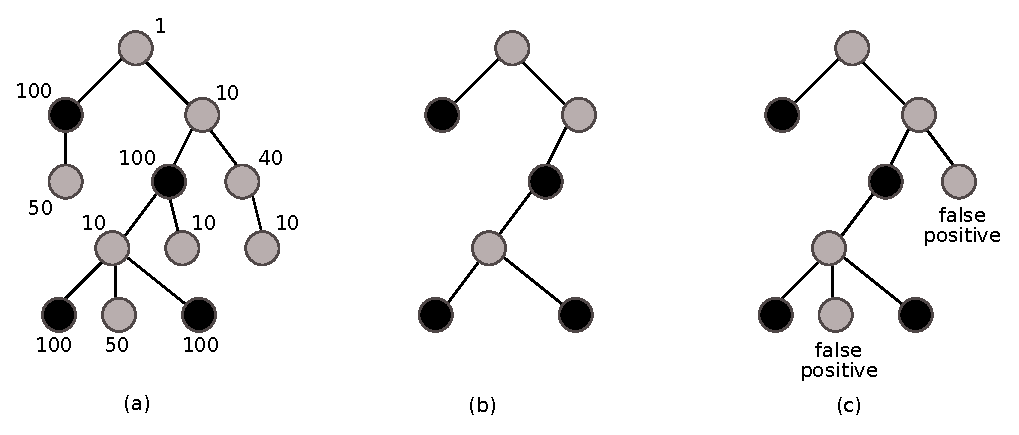
\includegraphics[width=0.95\columnwidth]{figures/hcct-example/hcct-example.eps}
\caption{\protect\label{fig:hcct-example} (a) CCT annotated with calling-context frequency counts; (b) HCCT; and (c) $(\phi,\varepsilon)$-HCCT. Hot nodes are black. In this example $N=581$, $\phi=1/10$, and $\varepsilon=1/30$: the approximate HCCT includes all contexts with frequency $\ge\lfloor\phi N\rfloor=58$  and no context with frequency $\le\lfloor(\phi-\varepsilon) N\rfloor=38$.
}
\end{center}
\end{figure}
\fi

\paragraph*{A Data Streaming Problem.} The execution trace of routine invocations and terminations can be naturally regarded as a stream of items. Each item is a triple containing routine name, call site, and event type (i.e., routine invocation or termination). Figures reported in \mytable\ref{tab:hcct-CCTsize} indicate that the number of distinct routines (i.e., the number of nodes of the call graph) is small compared to the stream length (i.e., to the number of nodes of the call tree), even for complex applications. Hence, non-contextual profilers -- such as vertex profilers -- can easily collect performance metrics for all the routines using a hash table. This may not be sustainable in the case of contextual profiling, when the number of distinct calling contexts (i.e., the number of CCT nodes) is too large and hashing would be inefficient. Motivated by the fact that execution traces are typically very long and their items (calling contexts) are taken from a large universe, we cast the problem of identifying the most frequent contexts into a data streaming setting.

In the data streaming computational model, algorithms should be able to perform near-real time analyses on massive data streams, where input data come at a very high rate and cannot be stored entirely due to their huge, possibly unbounded size~\cite{Demetrescu07,Muthukrishnan05}. This line of research has been mainly motivated by networking and database applications: for instance, a relevant IP traffic analysis task consists of monitoring the packet log over a given link in order to estimate how many distinct IP addresses used that link in a given period of time. Space-efficient data streaming algorithms can maintain a compact data structure that is dynamically updated upon arrival of new input data, supporting a variety of application-dependent queries. Approximate answers are allowed when it is impossible to obtain an exact solution using only limited space. Streaming algorithms are therefore designed to optimize space usage and update/query time while guaranteeing high solution quality.

\paragraph*{Finding Frequent Items in a Stream.} The problem of computing the HCCT online can be reconducted to the {\em frequent items} (a.k.a. heavy hitters) problem, which has been extensively studied in the data streaming model. Given a frequency threshold $\phi\in[0,1]$ and a stream of length $N$, the problem (in its simplest formulation) is to find all items that appear in the stream at least $\lfloor\phi N\rfloor$ times, i.e., having frequency $\ge\lfloor\phi N\rfloor$. For instance, for $\phi=0.1$ the problem seeks all items that appear in the stream at least $10\%$ of the times. Notice that at most $1/\phi$ items can have frequency larger than $\lfloor\phi N\rfloor$.  It can be proved that any algorithm that outputs an exact solution requires $\Omega(N)$ bits, even using randomization~\cite{Muthukrishnan05}. Note that this lower bound result extends to the problem of computing the HCCT, which thus cannot be calculated exactly in a space asymptotically smaller than the entire CCT. Hence, researchers have focused on solving an approximate version of the problem:

\begin{definition} 
{\mbox{$(\phi,\varepsilon)$-heavy hitters problem.}} Given two parameters $\phi,\varepsilon\in[0,1]$, with $\varepsilon<\phi$, an algorithm has to return all items with frequency $\ge\lfloor\phi N\rfloor$ and no item with frequency $\le\lfloor(\phi-\varepsilon) N\rfloor$.
\end{definition} 

\noindent In the approximate solution, false negatives are not allowed, i.e., all frequent items must be returned. Instead, some false positives can exist, but their actual frequency is guaranteed to be at most $\varepsilon N$-far from the threshold $\lfloor\phi N\rfloor$. For the HCCT construction, we focus on a variant of the problem where, besides returning the heavy hitters, it is necessary to estimate accurately their true frequencies, the stream length $N$ is not known in advance, and all the items in the stream have equal weight.

Counter-based streaming algorithms solve this problem by tracking a subset of items from the input and monitoring counts associated with them. For each new arrival, these algorithms decide whether to store the item or not, and, if so, what counts to associate with it. Update times are typically dominated by a small (constant) number of dictionary or heap operations. These algorithms, according to extensive experimental studies~\cite{Cormode08}, have superior performance with respect to space, running time, and accuracy compared to other classes of algorithm for $(\phi,\varepsilon)$-heavy hitters that have been proposed in the literature in the last 15 years.

\paragraph*{Approximate HCCT.} Streaming algorithms for mining frequent items can be used to solve a relaxed version of the HCCT construction problem. We thus compute an {\em Approximate Hot Calling Context Tree} that we denote by {\em $(\phi,\varepsilon)$-HCCT}, where $\varepsilon<\phi$ controls the degree of approximation:

\begin{definition}
Given a set A of $(\phi,\varepsilon)$-heavy hitters, the {\em $(\phi,\varepsilon)$-HCCT} is the minimal subtree of the CCT spanning all the nodes in A and the CCT root.
\end{definition}

\noindent A $(\phi,\varepsilon)$-HCCT contains all hot nodes (true positives), but may possibly contain some cold nodes without hot descendants (false positives). The true frequency of these false positives, however, is guaranteed to be at least $\lfloor(\phi-\varepsilon) N\rfloor$. Unlike the HCCT, a $(\phi,\varepsilon)$-HCCT is not uniquely defined, since the set of $(\phi,\varepsilon)$-heavy hitters is not unique: nodes with frequencies smaller than $\lfloor\phi N\rfloor$ and larger than $\lfloor(\phi-\varepsilon) N\rfloor$ may be either in such a set or not depending on the streaming algorithm being used. On the other hand, the HCCT is always a subtree of any $(\phi,\varepsilon)$-HCCT.

\ifdefined\noauthorea
\begin{figure}[ht]
\begin{center}
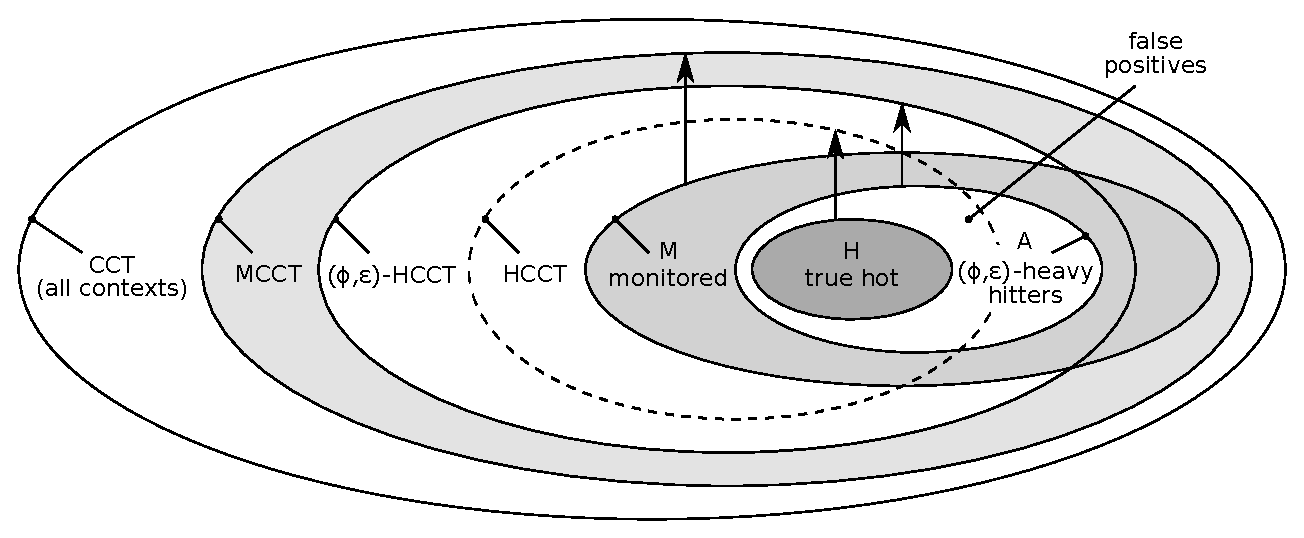
\includegraphics[width=0.95\columnwidth]{figures/hcct-venn/hcct-venn.eps}
\caption{\protect\label{fig:hcct-venn} Tree data structures and calling contexts classification. Graphical notation S $\uparrow$ T indicates that T is the minimal subtree of the CCT spanning all nodes in S.
}
\end{center}
\end{figure}
\fi

\subsection{Algorithms}
\label{ss:hcct-algorithms}

Computing a $(\phi,\varepsilon)$-HCCT online requires extending the canonical CCT construction algorithm with an online pruning strategy, which is implicitly driven by the actions of an underlying streaming algorithm. Constructing a CCT on-the-fly during the execution of a program is a straightforward task. Let $v$ be a cursor pointer that points to the current context, i.e., to the node corresponding to the calling context of the currently active routine ($v$ is initialized to the CCT root node). At each routine invocation, the algorithm checks whether $v$ has a child associated with the called routine. If this is the case, the existing child is used and its metrics are updated, if needed. Otherwise, a new child of $v$ is added to the CCT. In both cases, the cursor is moved to the callee. Upon routine termination, the cursor is moved back to the parent node in the CCT. Note that this approach can be implemented either by instrumenting every routine call and return or by performing stack-walking if sampling is used to inhibit redundant profiling~\cite{Arnold00,Whaley00,Zhuang06}.

In order to computer the set A of $(\phi,\varepsilon)$-heavy hitters, counter-based streaming algorithms need to monitor a slightly larger set M$\,\supseteq\,$A of elements. Nodes in M$\,\setminus\,$A can be either ancestors of nodes in A and thus already in the $(\phi,\varepsilon)$-HCCT, or nodes not in the $(\phi,\varepsilon)$-HCCT; for the latter category, we have to retain information about their ancestors as well, which might not be in the $(\phi,\varepsilon)$-HCCT. We denote as MCCT the minimal subtree of the CCT spanning all the nodes in M and the CCT root. \myfigure\ref{fig:hcct-venn} graphically illustrates the relationships among all our data structures.

Our $(\phi,\varepsilon)$-HCCT construction algorithm has to maintain the MCCT dynamically while the underlying algorithm processes the execution trace and updates M. At query time, the streaming algorithm analyzes M to discard all the elements in M$\,\setminus\,$A: the MCCT is thus pruned appropriately and the $(\phi,\varepsilon)$-HCCT$\,\subseteq\,$MCCT is returned.

\paragraph*{An Example.} To understand why the heavy hitters and the approximate HCCT are not maintained directly, but derived by pruning M and MCCT, respectively, we discuss a scenario where M is larger than the number of heavy hitters. Consider the following example: the execution trace contains the initial invocation of the {\tt main} function, which in turn invokes once a routine $p$, and $N-2$ times a different routine $q$. Hence, we have three distinct calling contexts: {\tt main}, {\tt main}$\rightarrow${\tt p}, and, {\tt main}$\rightarrow${\tt q}. Assume that $N\ge 8$, $\varepsilon=1/4$, $\phi=1/2$, and that the counter-based streaming subroutine can maintain three counters, one for each calling context. Then, only context {\tt main}$\rightarrow${\tt q} has frequency larger than $\lfloor(\phi-\varepsilon)N\rfloor$ and is a $(\phi,\varepsilon)$-heavy hitter, but -- as we assumed there is room in M for all contexts -- a streaming algorithm can maintain the exact frequencies of both {\tt main}$\rightarrow${\tt p} and {\tt main}$\rightarrow${\tt q}. Since {\tt main}$\rightarrow${\tt p} has frequency 1, it would be an error returning it as a heavy hitter. For this reason, M needs to be post-processed in order to eliminate low-frequency items that may be included when there are more available counters than heavy hitters.

\paragraph*{Data Structure Operations.} At each function call, the set M of monitored contexts is updated by a counter-based streaming algorithm. When M is changed, the subtree MCCT spanning nodes in M needs to be brought up to date as well. To describe how this happens, we assume that the interface of the streaming algorithm provides two main functions:

%TODO fix alignment
%\begin{enumerate}[align=left,leftmargin=*]
\begin{description}
\item[{\tt update(x,M)}$\rightarrow\,${\tt V}] Given a calling context $x$, update M to reflect the new occurrence of $x$ in the stream (e.g., if $x$ was already monitored in M, its frequency count may be increased by one). This function might return a set V of {\em victim} contexts that were previously monitored in M and are evicted during the update (as a special case, $x$ itself may be considered as a victim if the algorithm chooses not to monitor it).
\item[{\tt query(M)}$\rightarrow\,${\tt A}] Remove low-frequency items from M and return the subset A of $(\phi,\varepsilon)$-heavy hitters (see \myfigure\ref{fig:hcct-venn}).
\end{description}
%\end{enumerate}

\ifauthorea{}{\par\begingroup \parfillskip 0pt \relax}
\noindent As with the CCT, during the construction of the MCCT we maintain a cursor pointer that points to the current calling context, creating a new node if the current context $x$ is encountered for the first time. Additionally, we prune the MCCT according to the victim contexts returned by the streaming {\tt update} operation (these contexts are no longer monitored in M). The pseudocode of the pruning algorithm is given in \myalgorithm\ref{alg:hcct-update}. Since the tree must remain connected, victims can be removed from
\ifauthorea{}{\par\endgroup}
\ifdefined\noauthorea

\begin{figure}[h!]
\IncMargin{2em}
\begin{algorithm}[H]
\LinesNumbered
\SetAlgoNoLine
\SetNlSkip{1.5em} 
\Indm\Indmm
\nonl\hrulefill\\
\KwIn{MCCT; node $x$ to be pruned.}
\KwOut{Pruned MCCT.}
\vspace{-2mm}\hrulefill\\
\Indp\Indpp
$V$ $\gets$ {\tt update}(x, M);\\
\ForEach{context $v\in V\,\backslash \{x\}$}{
    \While{$(v$ is a leaf in MCCT$)$ $\wedge$ $(v\not\in$ M$)$}{
        remove $v$ from MCCT\\
        $v$ $\gets$ parent$(v)$
    }
}
\vspace{-2mm}
\Indm\Indmm
\nonl\hrulefill\vspace{1mm}\\
\DecMargin{2em}
\caption{\label{alg:hcct-update} Online pruning algorithm for MCCT construction.}
\end{algorithm}
\end{figure}


\noindent
\fi
the MCCT only if they are leaves. Moreover, removing a victim might expose a path of unmonitored ancestors that no longer have descendants in M: these nodes are pruned as well. The node for the current context $x$ is never removed from the MCCT, even if the context is not necessarily monitored in M. This guarantees that no node in the path from the tree root to $x$ will be removed: these nodes have at least $x$ as a descendant and the leaf test (line 3 in \myalgorithm\ref{alg:hcct-update}) will always fail.
A similar pruning strategy can be used to compute the $(\phi,\varepsilon)$-HCCT from the MCCT. The streaming {\tt query} operation is first invoked on M, returning the support A of the $(\phi,\varepsilon)$-HCCT. All MCCT nodes that have no descendant in A are then removed, following bottom-up path traversals as in the prune operation.

\ifx\noauthorea\undefined
\begin{figure}[ht]
\caption{\label{alg:hcct-update} Online pruning algorithm for MCCT construction.}
\begin{small}
\begin{minipage}{0.9\textwidth}
\hrulefill\\
\textbf{Input}: {MCCT; node $x$ to be pruned.}\\
\textbf{Output}: {Pruned MCCT.}

\vspace{-1mm}
\hrulefill\\
1. ~~ $V$ $\gets$ {\tt update}(x, M);\\
2. ~~ \textbf{foreach} context $v\in V\,\backslash \{x\}$ \textbf{do}\\
3. ~~ ~~~~ \textbf{while} $(v$ is a leaf in MCCT$)$ $\wedge$ $(v\not\in$ M$)$ \textbf{do}\\
4. ~~ ~~~~ ~~~~ remove $v$ from MCCT\\
5. ~~ ~~~~ ~~~~ $v$ $\gets$ parent$(v)$\\
6. ~~ ~~~~ \textbf{end}\\
7. ~~ \textbf{end}

\vspace{-1mm}
\hrulefill
\vspace{-2mm}
\end{minipage}
\end{small}
\end{figure}
\fi

%Algorithmic details on updating and querying M and MCCT are given in \mysection\ref{ss:hcct-algorithms}.

%\subsection{Implementation}

\subsection{Comparison with Related Work}

CCTs have been introduced in~\cite{Ammons97} as a practical data structure to associate performance metrics with paths through a program's call graph: Ammons, Ball, and Larus suggest to build a CCT by instrumenting procedure code and to compute metrics by exploiting hardware counters available in modern processors. It has been later observed, however, that exhaustive instrumentation can incur large slowdowns.

\paragraph*{Reducing Overhead.} To reduce the overhead from instrumentation, in~\cite{Bernat07} the authors generate path profiles including only methods of interest, while statistical profilers~\cite{Arnold00,Froyd05,Hall93,Whaley00} attribute metrics to calling contexts through periodic sampling of the call stack. For call-intensive programs, sample-driven stack-walking can be orders of magnitude faster than exhaustive instrumentation, but may incur significant loss of accuracy with respect to the complete CCT: sampling guarantees neither high coverage~\cite{Bond07} nor accuracy of performance metrics~\cite{Zhuang06}, and its results may be highly inconsistent in different executions.

A variety of works explores the combination of sampling with bursting~\cite{Arnold01,Hirzel01,Zhuang06}. Most recently, Zhuang {\em et al.} suggest to perform stack-walking followed by a burst during which the profiler traces every routine call and return~\cite{Zhuang06}: experiments show that adaptive bursting can yield very accurate results. In~\cite{Serrano09}, the profiler infrequently collects small call traces that are merged afterwards to build large calling context trees: ambiguities might emerge during this process, and the lack of information about where the partial CCTs should be merged to does not allow reconstructing the entire CCT univocally.

The main goal of all these works is to reduce profiling overhead without incurring significant loss of accuracy. Our approach is orthogonal to this line of research and regards space efficiency as an additional resource optimization criterion besides profile accuracy and time efficiency. When the purpose of profiling is to identify hot contexts, exhaustive instrumentation, sampling, and bursting might all be combined with our approach and benefit of our space reduction technique.

In a recent work~\cite{Huang13}, a novel data structure is proposed to avoid the node lookup operation in dynamic bug detectors. A new node is instead allocated for each context, and the costs of allocations are mitigated by extending the garbage collector not only to collect unused node, but also to merge duplicate ones lazily.

\paragraph*{Reducing Space.} A few previous works have addressed techniques to reduce profile data (or at least the amount of data presented to the user) in context sensitive profiling. Incremental call-path profiling lets the user choose a subset of routines to be analyzed~\cite{Bernat07}. Call path refinement helps users focus the attention on performance bottlenecks by limiting and aggregating the information revealed to the user~\cite{Hall95}. These works are quite different in spirit from our approach, where only hot contexts are profiled and identified automatically during program's execution.

Probabilistic calling contexts have been introduced as an extremely compact representation (just a 32-bit value per context), especially useful for tasks such as residual testing, statistical bug isolation, and anomaly-based intrusion detection~\cite{Bond07}. Bond and McKinley target applications where coverage of both hot and cold contexts is necessary, but their inspection is unnecessary. This is not the case in performance analysis, where identifying and understanding a few hot contexts is typically sufficient to guide code optimization. Hence, although sharing with~\cite{Bond07} the common goal of space reduction, our approach targets a rather different application context.

Somner et al. proposed a technique called {\em Precise Calling Context Encoding} (PCCE) that encodes acyclic paths in the call graph of a program into one number, while recursive call paths are divided into acyclic subsequences and encoded independently~\cite{Sumner12}. Different calling contexts are guaranteed to have different IDs that can be faithfully decoded, and experiments on a prototype implementation for C programs show negligible overhead. However, PCCE would not work in the presence of virtual methods and dynamic class loading in object-oriented languages, and the encoding scheme shows scalability problems when handling large-scale software~\cite{Bond10,Zeng14}. These limitations, which are absent from our solution, have been recently addressed in~\cite{Zeng14}, and it would be interesting to investigate whether their approach can be extended to collect performance metrics and in turn filter the collected data on-the-fly using a data streaming approach as we do in this work.

%~\cite{}

\subsection{Discussion}

% dire dello spazio asintoticamente minore